\documentclass[10pt,tikz,border=10pt]{standalone}
%\usepackage[utf8]{inputenc}
\usepackage[T1]{fontenc}
\usepackage{amsmath}
%\usepackage{amsfonts}
\usepackage{amssymb}
\usepackage{mathtools}
\DeclarePairedDelimiter\abs{\lvert}{\rvert}
\usepackage{tikz}
\usetikzlibrary{shapes,arrows,shapes.misc,shapes.symbols}
\usetikzlibrary{positioning}
\usepackage{gitinfo2}
%\usepackage{graphicx}

\makeatletter
\AddToShipoutPictureBG{%
	\AtPageLowerLeft{%
		\kern2.6cm
		\raisebox{\dimexpr.5\paperheight-.8\height}
		{\rotatebox{90}{\gitMarkFormat\gitMarkPref{} \textbullet{} \gitMark}}%
	}%
}%
\makeatother
\newcommand{\prdfrazioni}{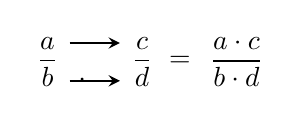
\begin{tikzpicture}[thick]
		\def\x{2.8mm}
		\def\h{2.4mm}
		\def\dist{12mm}%1cm
		\node at (0,0) {$\displaystyle \frac{a}{b}$};
		\node at (\dist,0) {$\displaystyle \frac{c}{d}$};
		\node at (1.4*\dist,0) {$\displaystyle =$};
		\node at (2.0*\dist,0) {$\displaystyle \frac{a\cdot c}{b\cdot d}$};
		% collegamento termini
		\draw[-stealth] (\x, \h)--(\dist-\x,\h); 
		\draw[-stealth] (\x,-\h)--node [near start] {$\cdot$}(\dist-\x, -\h);
	\end{tikzpicture}%
}
%\renewcommand{\gitMarkFormat}{\color{blue}\sffamily\bfseries}
\begin{document}
\tikzset{
	decision/.style={diamond, draw, %fill=blue!20,
		text width=5.5em, text badly centered, 
	%	node distance=1.8cm
		, inner sep=0pt
	},
	block/.style={rectangle, draw, %fill=blue!20,
	%	text width=15em, 
		text centered, 
		%node distance=2.0cm,
		%rounded corners, 
		%minimum height=3em
	},
commento/.style={draw=black!20!white, line width=1pt, dash pattern=on 1pt off 
4pt on 6pt off 4pt,
%	inner ysep=6mm,inner xsep=1mm, 
	rectangle,
%	 rounded corners
 },
	loop/.style={chamfered rectangle,chamfered rectangle 	xsep=2cm, draw, %fill=blue!20,
		text width=15em, text centered,  
		node distance=2.5cm,% minimum height=3em
	},
	cloud/.style={draw, ellipse,%fill=red!20, 
		%node distance=1.5cm,
		 minimum height=2em
	},
	input/.style={ % requires library shapes.geometric
		draw,
		%node distance=1.5cm,
			%text width=15em, 
			text centered,  
		trapezium,
		trapezium left angle=60,
		trapezium right angle=120,
	},
	line/.style={draw, very thick, %color=black!50,
		-latex'},
	print/.style={ % requires library shapes.symbols
		draw,
		%text width=14em, 
		text centered,  
		tape,
		tape bend top=none
	},
connessione/.style={
draw,
circle,
radius=5pt,
}
}

		\begin{tikzpicture}[scale=1, %node distance = 2.5cm,
			 auto]
			% Place nodes
			\node [cloud] (init) {Inizio};
			\node [block, below of=init] (1) {$ax^2+bx+c=0$};
			\node [input,below of=1,text width=35em,node 
			distance=1.5cm](2){$a$ è il numero 
			del termine di 
			secondo grado, $b$ è il numero del termine di primo grado, $c$ il 
			termine di grado zero, i termini mancanti valgono zero };

		\node[block,below of=2,node distance=1.5cm] (3) {$\Delta=b^2-4ac$}; 
		\node[decision,below of=3,node distance=2.5 cm] (4) {$\Delta<0$};
		\node[print,below right=0.5cm and 1.6cm of 4,text width=5em, ] (5) 		
		{Non ho soluzioni reali};
		\node[decision,below left=1cm and 2.0cm of 4] (6) {$\Delta=0$};
		\node[print,below right=0.5cm and 1.6cm of 6,text width=5em, ] (7) 
		{Ho soluzioni coincidenti};
		\node[print,below left=0.5cm and 1.6cm of 6,text width=5em, ] (8) 
		{Soluzioni distinte};
		\node[print,below of=7 ,node distance=2.5 cm] (9) 
		{$x_{1,2}=-\dfrac{b}{2a}$};
		\node[print,below of=8 ,node distance=2.5 cm] (10) 
		{$x_{1,2}=\dfrac{-b\pm\sqrt{\Delta}}{2a}$};
		\node[connessione,below of=6,node distance=2cm] (11) at (10 -| 6){}; 
		\node[connessione,below of=12,node distance=3cm] (12) at (16 -| 4){};
%		\node[connessione,below of=12,node distance=5cm] (21) at (16 -| 2){};  
%		\node [cloud,below of=21,node distance=2cm] (stop) {Fine};
			\path [line] (init) -- (1);
     		\path [line] (1) --  (2);
     		\path [line] (2) --  (3);
     		\path [line] (3) --  (4);
    		\path [line] (4.west) -- node[near start] {No}++(-2,0)-|    		
    		(6.north);
     		\path [line] (4.east) -- node[near start] {Si}++(2,0)-| (5.north);
    		\path [line] (6.east) -- node[near start] {Si}++(2,0)-| (7.north);
     		\path [line] (6.west) -- node[near start] {No}++(-2,0)-| 
     		(8.north);
    		\path [line] (7) --  (9);
    		\path [line] (8) --  (10);
     		\path [line] (10.south) -- ++(0,-1)|- (11);
     		\path [line] (9.south) -- ++(0,-1)|- (11);
%     		\path [line] (19.south) -- ++(0,-1)|- (20);
%     		\path [line] (13.south) -- ++(0,-1)|- (20);
%     		\path [line] (20.south) -- ++(0,-1)|- (21);
%     		\path [line] (9.south) -- ++(0,-1)|- (21);
%     		\path [line] (21) --  (stop);
		\end{tikzpicture}
\end{document}